
% xetex expected
\documentclass[xetex,professionalfont]{beamer}

% we want math
\usepackage{amsmath}

% fixes and extensions to amsmath
\usepackage{mathtools}

% additional math symbols
\usepackage{amssymb}

% good-looking fractions in text via \sfrac
\usepackage{xfrac}

% fix spaces after custom commands (see below for examples)
\usepackage{xspace}

% minted allows for fancy syntax highlighting (requires python with pygments)
% usage:
%   \begin{minted}{python}
%   codeb
%   \end{minted}
\usepackage{minted}

% better looking tables
% usage:
%   begin with a \toprule, write a single row of column headings,
%   then add \midrule and after the columns of data we finish with \bottomrule
% example:
%   \begin{tabular}{llr} \toprule
%   Animal & Description & Price \midrule
%   cat & foo & 10 \\
%   dog & bar & 20 \\ \bottomrule
%   \end{tabular}
% note that good tables generally neither have vertical rules nor double rules
\usepackage{booktabs}

% system font support (requires xetex or luatex)
\usepackage{fontspec}
\setmonofont[Scale=0.7]{Cousine} % part of ttf-chromeos fonts on Arch

% multi-language quotes for babel
\usepackage{csquotes}

% easy way to include copyright information
\usepackage{copyrightbox}

% better bibliographies
\usepackage[backend=biber,style=authoryear]{biblatex}

% language support (english,ngerman)
\usepackage[english]{babel}

% minted screws up line spacings ...
\usepackage{setspace}
\usepackage{enumitem}

% -----------------------------------------------------------------------------

% specify PDF metadata
\hypersetup{pdftitle={CVSP VO - Specific Object Recognition},pdfsubject={},pdfauthor={Christopher Pramerdorfer}}

% copyright font style
\makeatletter\renewcommand{\CRB@setcopyrightfont}{\tiny\color{lightgray}}

% add bib file
\addbibresource{literature.bib}

% use tuwcvl beamer theme
\usetheme{tuwcvl}

% add some space between lines
\setstretch{1.4}

% but not for minted environments
\AtBeginEnvironment{minted}{\singlespacing}

% fix itemize

\setlist{nolistsep}
\setitemize{itemsep=-1mm,label=\usebeamerfont*{itemize item}%
  \usebeamercolor[fg]{itemize item}
  \usebeamertemplate{itemize item}}

% -----------------------------------------------------------------------------

% common english abbreviations
\newcommand{\ie}{\mbox{i.e.}\xspace} % i.e.
\newcommand{\eg}{\mbox{e.g.}\xspace} % e.g.

% math - argmin and argmax
\DeclareMathOperator*{\argmin}{arg\,min}
\DeclareMathOperator*{\argmax}{arg\,max}

% shortcuts for number ranges
\newcommand{\NN}{\mathbb{N}}
\newcommand{\ZZ}{\mathbb{Z}}
\newcommand{\QQ}{\mathbb{Q}}
\newcommand{\RR}{\mathbb{R}}

% bold vectors
\renewcommand{\vec}[1]{\ensuremath{\mathbf{#1}}}

% vector shortcuts
\newcommand{\va}{\vec{a}}
\newcommand{\vb}{\vec{b}}
\newcommand{\vc}{\vec{c}}
\newcommand{\ve}{\vec{e}}
\newcommand{\vr}{\vec{r}}
\newcommand{\vs}{\vec{s}}
\newcommand{\vt}{\vec{t}}
\newcommand{\vu}{\vec{u}}
\newcommand{\vv}{\vec{v}}
\newcommand{\vw}{\vec{w}}
\newcommand{\vx}{\vec{x}}
\newcommand{\vy}{\vec{y}}
\newcommand{\vz}{\vec{z}}

\newcommand{\bth}{\boldsymbol{\theta}}
\newcommand{\intr}{\boldsymbol{\Lambda}}

% highlight
\newcommand{\highlight}[1]{\textcolor{tuwcvl_inf_red}{\textbf{#1}}}

% make emph red
\let\oldemph\emph
\renewcommand\emph[1]{\textcolor{tuwcvl_inf_red}{#1}}

% -----------------------------------------------------------------------------

\title{Computer Vision Systems Programming VO}
\subtitle{Specific Object Recognition}
\author{Christopher Pramerdorfer}
\institute{Computer Vision Lab, Vienna University of Technology}

\begin{document}

% -----------------------------------------------------------------------------

\begin{frame}
\maketitle
\end{frame}

% -----------------------------------------------------------------------------

\begin{frame}
\frametitle{Topics}

Introduction to object recognition \\
Specific object recognition

\bigskip
\begin{center}
    \copyrightbox[b]
    {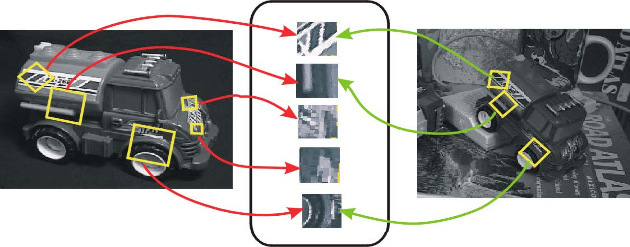
\includegraphics[width=7cm]{figures/local-feature-matching.jpg}}
    {\centering Image from \cite{grauman2011}}
\end{center}

\end{frame}

% -----------------------------------------------------------------------------

\begin{frame}
\frametitle{Object Recognition}

Fundamental problem in Computer Vision

\bigskip
Many applications
\begin{itemize}
	\item Panorama stitching, 3D reconstruction
	\item HCI and surveillance (face recognition)
	\item Image understanding (recall Fei-Fei Li's TED talk)
\end{itemize}

\end{frame}

% -----------------------------------------------------------------------------

\begin{frame}
\frametitle{Object Recognition}
\framesubtitle{Taxonomy -- Instance vs.\ Category}

\emph{Instance recognition} (\emph{specific object recognition})
\begin{itemize}
	\item Recognize a specific, uniquely looking object % even if differences are only in details
	\item Face of a certain person, the Eiffel tower
\end{itemize}

\bigskip
\emph{Object category recognition}
\begin{itemize}
	\item Recognize objects of a certain category % note that categories are hierarchical ... like panda bears - bears - mammals - animals. some test databases reflect this, like ImageNet. obviously, the more general the category, the harder the recognition task
	\item Human faces, buildings
\end{itemize}

\end{frame}

% -----------------------------------------------------------------------------

\begin{frame}
\frametitle{Object Recognition}
\framesubtitle{Taxonomy -- Instance vs.\ Category}

\begin{center}
\begin{tikzpicture}
    \node[anchor=south west,inner sep=0] (image) at (0,0) {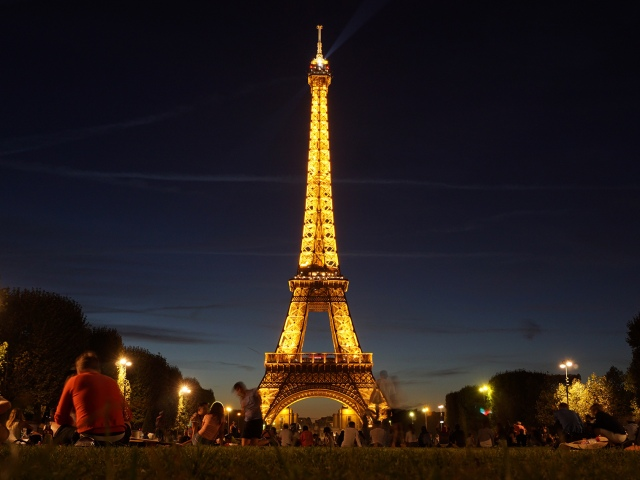
\includegraphics[width=8cm]{figures/eiffel-tower.jpg}};
    \begin{scope}[x={(image.south east)},y={(image.north west)}]
        \node[green] at (0.205,0.94) {category: building};
        \node[green] at (0.24,0.87) {instance: Eiffel tower};
    \end{scope}
\end{tikzpicture}
\end{center}

\end{frame}

% -----------------------------------------------------------------------------

\begin{frame}
\frametitle{Object Recognition}
\framesubtitle{Taxonomy -- Classification vs.\ Detection}

\emph{Object classification}
\begin{itemize}
	\item Recognize main object in image % disregarding the rest / we assume that there is a dominant object in the image (maybe we detected the object and cropped the image in a preprocessing step)
	\item Location and other objects not relevant
\end{itemize}

\bigskip
\emph{Object detection}
\begin{itemize}
	\item Recognize multiple objects, possibly of different category
\end{itemize}

\end{frame}

% -----------------------------------------------------------------------------

\begin{frame}
\frametitle{Object Recognition}
\framesubtitle{Taxonomy -- Classification vs.\ Detection}

\begin{center}
\begin{tikzpicture}
    \node[anchor=south west,inner sep=0] (image) at (0,0) {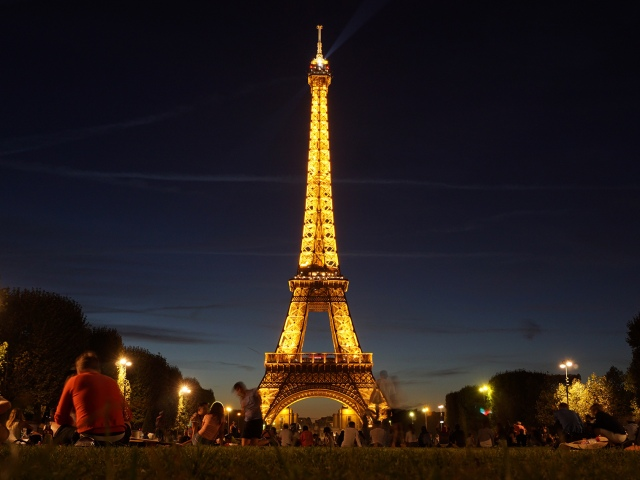
\includegraphics[width=8cm]{figures/eiffel-tower.jpg}};
    \begin{scope}[x={(image.south east)},y={(image.north west)}]
        \draw[red,ultra thick] (0.35,0.08) rectangle (0.65,0.97);
        \node[red] at (0.75,0.54) {building};
        \draw[red,ultra thick] (0.08,0.08) rectangle (0.21,0.28);
        \node[red] at (0.145,0.32) {person};
        \node[green] at (0.1,0.94) {building}; % the class of the image (classification task)
    \end{scope}
\end{tikzpicture}
\end{center}

\end{frame}

% -----------------------------------------------------------------------------

\begin{frame}
\frametitle{Object Recognition}
\framesubtitle{Challenges}

Instances of same category can look very differently
\begin{itemize}
    \item Illumination, pose, viewpoint, occlusions, background
\end{itemize}

\medskip
\begin{center}
    \copyrightbox[b]
    {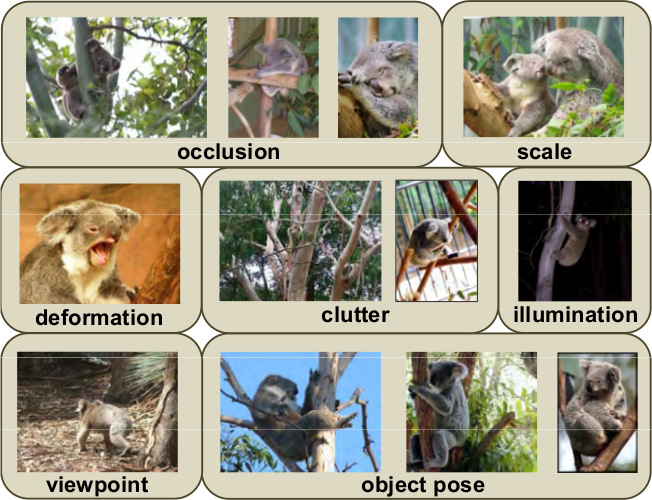
\includegraphics[width=6cm]{figures/challenges.jpg}}
    {\centering Image from \cite{grauman2011}}
\end{center}

\end{frame}

% -----------------------------------------------------------------------------

{
\setbeamertemplate{footline}{}
\begin{frame}

\begin{tikzpicture}[remember picture,overlay]
\fill[white] (current page.north west) rectangle (current page.south east);
\end{tikzpicture}

\end{frame}
}

% -----------------------------------------------------------------------------

\begin{frame}
\frametitle{Planar Rigid Object Detection}

We want to detect specific rigid planar objects
\begin{itemize}
    \item Like markers, books
	\item Comparatively easy problem
\end{itemize}

\bigskip
Challenges
\begin{itemize}
	\item Unknown object pose and scale
	\item Varying illumination
    \item Partial occlusions
\end{itemize}

\end{frame}

% -----------------------------------------------------------------------------

\begin{frame}
\frametitle{Planar Rigid Object Detection}
\framesubtitle{Application: Marker-Based AR}

\begin{center}
    \copyrightbox[b]
    {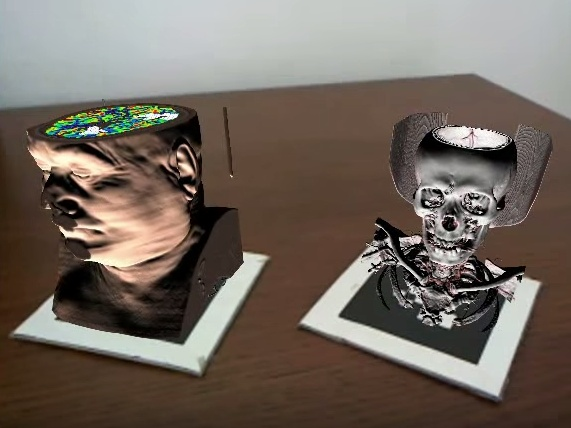
\includegraphics[width=7cm]{figures/marker-ar.jpg}}
    {\centering Image from \href{https://www.youtube.com/watch?v=ChGW2Jogdjs}{\texttt{youtube.com}}}
\end{center}

\end{frame}

% -----------------------------------------------------------------------------

\begin{frame}
\frametitle{Planar Rigid Object Detection}
\framesubtitle{Application: Panorama Stitching}

Assuming that object is far away (on \textit{plane at infinity})  % or if the camera undergoes a pure rotation

\medskip
\begin{center}
    \copyrightbox[b]
    {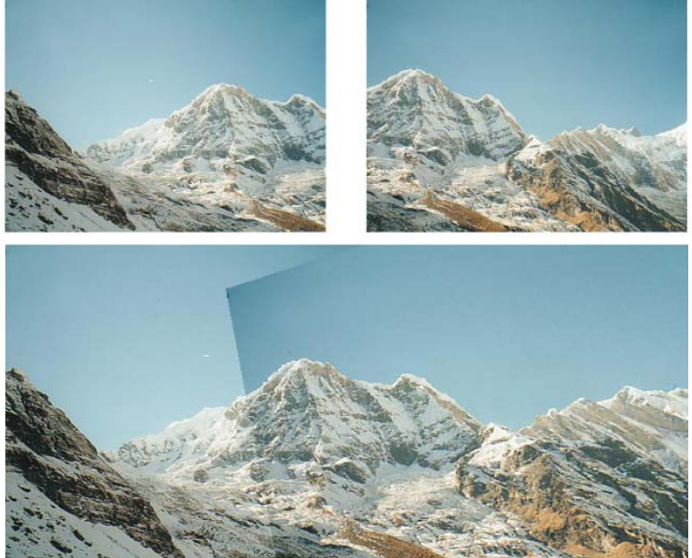
\includegraphics[width=6cm]{figures/panorama-stitching.jpg}}
    {\centering Image adapted from \cite{brown2007}}
\end{center}

\end{frame}

% -----------------------------------------------------------------------------

\begin{frame}
\frametitle{Planar Rigid Object Detection}
\framesubtitle{Selecting $\vx$ and $\vw$}

Our problem formulation is  % this is what is used normally because it is very flexible
\begin{itemize}
	\item Given a pixel location in a query image
	\item Predict location on object surface  % the unit will depend on the problem, like cm for pose estimation
\end{itemize}

\bigskip
So we know how to select $\vx$ and $\vw$
\begin{itemize}
	\item $\vx=(x,y)$ : pixel location in query image
	\item $\vw=(u,v)$ : corresponding location on object surface
\end{itemize}

\bigskip
As $\vw\in\RR^2$ this is a \emph{regression problem}

\end{frame}

% -----------------------------------------------------------------------------

\begin{frame}
\frametitle{Planar Rigid Object Detection}
\framesubtitle{Selecting $\vx$ and $\vw$}

\begin{center}
    \copyrightbox[b]
    {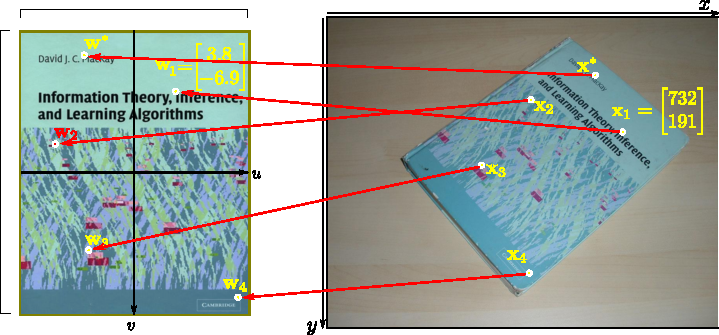
\includegraphics[width=10cm]{figures/book-pose.pdf}}
    {\centering Image adapted from \cite{prince12}}
\end{center}

\end{frame}

% -----------------------------------------------------------------------------

\begin{frame}
\frametitle{Planar Rigid Object Detection}
\framesubtitle{Model Selection}

Images of planar objects are always related by a \emph{homography} $\boldsymbol{\Phi}$
\begin{itemize}
	\item $3\times3$ matrix mapping between corresponding points
\end{itemize}

\bigskip
In homogeneous coordinates this means that
\[
	\lambda
	\begin{pmatrix}
		u \\ v \\ 1
	\end{pmatrix}
	= \boldsymbol{\Phi}
	\begin{pmatrix}
		x \\ y \\ 1
	\end{pmatrix}
\]

\end{frame}

% -----------------------------------------------------------------------------

\begin{frame}
\frametitle{Planar Rigid Object Detection}
\framesubtitle{Model Selection}

The model of choice is thus (disregarding noise)  % using Gamma below to represent the model as a function for next slide. this choice is arbitrary 
\[
	\vw=\Gamma(\vx)=
	\begin{pmatrix}
		u \\ v
	\end{pmatrix}\quad,\quad
	\lambda
	\begin{pmatrix}
		u \\ v \\ 1
	\end{pmatrix}
	= \boldsymbol{\Phi}
	\begin{pmatrix}
		x \\ y \\ 1
	\end{pmatrix}
\]

\end{frame}

% -----------------------------------------------------------------------------

\begin{frame}
\frametitle{Planar Rigid Object Detection}
\framesubtitle{Learning Model Parameters}

We again learn parameters $\bth$ from samples $\{(\vx_i,\vw_i)\}_{i=1}^n$
\begin{itemize}
	\item $\bth$ contains 9 parameters comprising $\boldsymbol{\Phi}$ % but 8 unknowns due to arbitrary scaling factor. we thus need n=4 points to find the parameters (if there is no noise)
\end{itemize}

\bigskip
Usually no exact solution because of noisy $\vx_i$
\begin{itemize}
	\item Formulate as a \emph{least squares problem} instead
\end{itemize}

\[
	\hat{\bth}=\argmin_{\bth} \left[\sum_{i=1}^n (\vw_i-\Gamma(\vx_i))^\top(\vw_i-\Gamma(\vx_i)) \right]
\]

\end{frame}

% -----------------------------------------------------------------------------

\begin{frame}
\frametitle{Planar Rigid Object Detection}
\framesubtitle{Learning Model Parameters}

This least squares approach is optimal
\begin{itemize}
	\item If noise is distributed normally with spherical covariance % with spherical covariance (same, independent noise affecting x1 and x2)
\end{itemize}

\bigskip
This is a nonlinear optimization problem
\begin{itemize}
	\item Solvable using any general nonlinear least squares solver % depends on a good initial estimate of the parameters (because there is no global optimum)
	\item OpenCV has an own function \texttt{findHomography}
\end{itemize}

\end{frame}

% -----------------------------------------------------------------------------

\begin{frame}
\frametitle{Planar Rigid Object Detection}
\framesubtitle{Pose Estimation}

$\boldsymbol{\Phi}$ is a 2D transformation

\bigskip
We may want to know the position and orientation of the object % or the position and orientation of the camera relative to the object
\begin{itemize}
    \item This is called \emph{pose estimation}
    \item Required e.g.\ for marker-based AR like above
\end{itemize}

\bigskip
This information can be extracted from $\boldsymbol{\Phi}$
\begin{itemize}
    \item If we know the intrinsic camera parameters % this can also be expressed by a 3x3 matrix
    \item See \cite{prince12} for details % if interested ... not required for the exam
\end{itemize}

\end{frame}

% -----------------------------------------------------------------------------

\begin{frame}
\frametitle{Planar Rigid Object Detection}
\framesubtitle{Obtaining Point Correspondences}

How can we compute $\{(\vx_i,\vw_i)\}_{i=1}^n$ automatically?
\begin{itemize}
    \item We first select $\vw_i$, then search corresponding $\vx_i$
\end{itemize}

\bigskip
$\vw_i$ can be selected
\begin{itemize}
    \item Manually (e.g.\ specific corners on markers)
    \item Automatically (e.g.\ SIFT)
\end{itemize}

\end{frame}

% -----------------------------------------------------------------------------

\begin{frame}
\frametitle{Planar Rigid Object Detection}
\framesubtitle{Obtaining Point Correspondences}

We opt for the second approach and use SIFT (or similar)
\begin{itemize}
    \item Features invariant to rotation, scale, illumination % this is nice given the challenges discussed
    \item Robust to affine transformations % to some extent. there are more suitable alternatives if there are strong transformations (like if we view the object from a sharp angle)
\end{itemize}

\bigskip
Approach
\begin{itemize}
    \item Compute keypoints and descriptors in both images
    \item Match descriptors (e.g.\ nearest neighbor association)
    \item Use keypoint locations of matches as $\{(\vx_i,\vw_i)\}_{i=1}^n$
\end{itemize}

\end{frame}

% -----------------------------------------------------------------------------

\begin{frame}
\frametitle{Planar Rigid Object Detection}
\framesubtitle{Obtaining Point Correspondences -- Remarks}

There will likely be incorrect matches
\begin{itemize}
    \item Would greatly impact the least squares solution
    \item Hence we use a robust alternative like RANSAC
\end{itemize}

\bigskip
\begin{center}
    \copyrightbox[b]
    {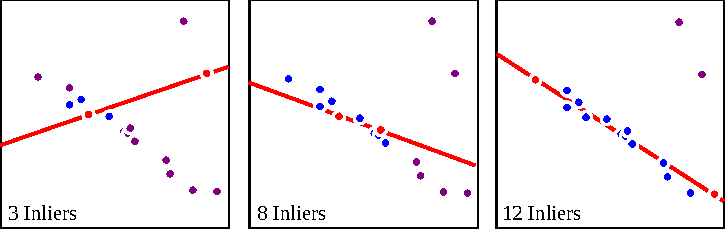
\includegraphics[width=9cm]{figures/ransac.pdf}}
    {\centering Image adapted from \cite{prince12}}
\end{center}

\end{frame}

% -----------------------------------------------------------------------------

\begin{frame}[fragile]
\frametitle{Planar Rigid Object Detection}
\framesubtitle{Obtaining Point Correspondences Using OpenCV}

\footnotesize
\begin{minted}{cpp}
// read images (SIFT expects grayscale images)
cv::Mat object = cv::imread("object.jpg", cv::IMREAD_GRAYSCALE);
cv::Mat search = cv::imread("search.jpg", cv::IMREAD_GRAYSCALE);

cv::SIFT sift; // using default arguments here

// compute keypoints
std::vector<cv::KeyPoint> kobject, ksearch;
sift.detect(object, kobject); sift.detect(search, ksearch);

// compute descriptors
cv::Mat dobject, dsearch;
sift.compute(object, kobject, dobject); sift.compute(search, ksearch, dsearch);
\end{minted}

\end{frame}

% -----------------------------------------------------------------------------

\begin{frame}[fragile]
\frametitle{Planar Rigid Object Detection}
\framesubtitle{Obtaining Point Correspondences Using OpenCV}

\footnotesize
\begin{minted}{cpp}
// find two nearest neighbors x,x' for each w
cv::FlannBasedMatcher matcher; // fast nearest neighbor search
std::vector<std::vector<cv::DMatch> > kMatches;
matcher.knnMatch(dobject, dsearch, kMatches, 2);

// keep match (x,w) if x is clearly more similar than x'
// this is a popular matching strategy
std::vector<cv::DMatch> matches;
for(const std::vector<cv::DMatch>& match : kMatches)
    if(match[0].distance < match[1].distance * 0.8) // x, x'
        matches.push_back(match[0]); // (x,w)
\end{minted}

\end{frame}

% -----------------------------------------------------------------------------

\begin{frame}[fragile]
\frametitle{Planar Rigid Object Detection}
\framesubtitle{Learning Homography Parameters Using OpenCV}

\footnotesize
\begin{minted}{cpp}
// collect feature locations of correspondences from before
std::vector<cv::Point2f> pobject, psearch;
for(const cv::DMatch& match : matches) { 
    pobject.push_back(kobject.at(match.queryIdx).pt);
    psearch.push_back(ksearch.at(match.trainIdx).pt);
}

// estimate homography using RANSAC for robustness
cv::Mat inliers; // contains indices of valid correspondences
cv::Mat homography = cv::findHomography(pobject, psearch, CV_RANSAC, 2, inliers);
\end{minted}

\end{frame}

% -----------------------------------------------------------------------------

{
\setbeamertemplate{footline}{}
\begin{frame}

\begin{tikzpicture}[remember picture,overlay]
\fill[white] (current page.north west) rectangle (current page.south east);
\end{tikzpicture}

\end{frame}
}

% -----------------------------------------------------------------------------

\begin{frame}
\frametitle{Nonplanar Rigid Object Detection}

\begin{center}
    \copyrightbox[b]
    {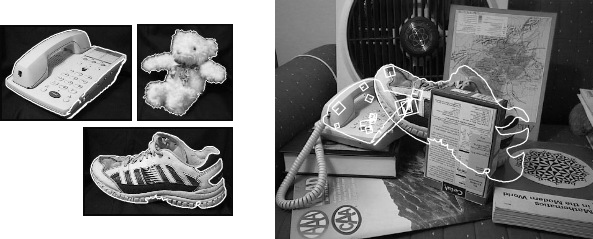
\includegraphics[width=9cm]{figures/rigid-object-detection.jpg}} % note the occlusions and transformations
    {\centering Image adapted from \cite{lowe2004}}
\end{center}

\end{frame}

% -----------------------------------------------------------------------------

\begin{frame}
\frametitle{Nonplanar Rigid Object Detection}

We use the same problem formulation as before
\begin{itemize}
    \item Given a pixel location in an image $\vx$
    \item Predict location on (nonplanar) object surface $\vw$
\end{itemize}

\bigskip
As object is no longer planar, we have $\vw=(u,v,w)$

\end{frame}

% -----------------------------------------------------------------------------

\begin{frame}
\frametitle{Nonplanar Rigid Object Detection}
\framesubtitle{Pinhole Camera Model}

How are $\vx$ and $\vw$ related in this case?
\begin{itemize}
    \item Let's recap the \emph{pinhole camera model} % we always assume this even though this is a simplification
\end{itemize}

\begin{center}
    \copyrightbox[b]
    {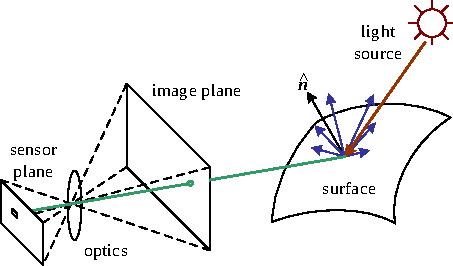
\includegraphics[width=7cm]{figures/image-formation.pdf}} % the pinhole camera model usually places the image plane in front of the pinhole for convenience, even though that's not physically possible.
    {\centering Image from \cite{szeliski2010}}
\end{center}

\end{frame}

% -----------------------------------------------------------------------------

\begin{frame}
\frametitle{Nonplanar Rigid Object Detection}
\framesubtitle{Pinhole Camera Model}

\begin{center}
    \copyrightbox[b]
    {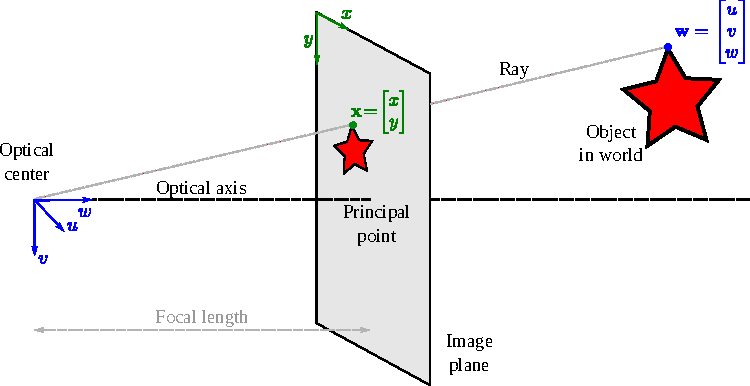
\includegraphics[width=9cm]{figures/pinhole-model.pdf}} % the model in the image is simplified in the sense that the camera is centered at the origin of the world coordinate system and because there is no skew
    {\centering Image adapted from \cite{prince12}}
\end{center}

\end{frame}

% -----------------------------------------------------------------------------

\begin{frame}
\frametitle{Nonplanar Rigid Object Detection}
\framesubtitle{Pinhole Camera Model}

% this applies only if the camera center is at the origin of the world coordinate system in which the object (and our w) resides, and if the image plane is parallel to the (u,v) plane. see next slide.

We see that in homogeneous coordinates % like before this is linear in homogeneous coordinates. it also looks similar, we just have a new coordinate w
\[
\lambda
\begin{pmatrix}
    x \\ y \\ 1
\end{pmatrix} =
\begin{pmatrix}
    f & 0 & p_x & 0 \\ 0 & f & p_y & 0 \\ 0 & 0 & 1 & 0
\end{pmatrix}
\begin{pmatrix}
    u \\ v \\ w \\ 1
\end{pmatrix}
\]

$f$ is the focal length in pixels \\
$p_x,p_y$ are the principal point coordinates

\end{frame}

% -----------------------------------------------------------------------------

\begin{frame}
\frametitle{Nonplanar Rigid Object Detection}
\framesubtitle{Pinhole Camera Model}

World and camera coordinate systems generally differ
\begin{itemize}
    \item Transform $\vw$ to camera coordinates before projection
\end{itemize}

\[
    \vw' =
    \begin{pmatrix}
        u' \\ v' \\ w'
    \end{pmatrix} =
    \begin{pmatrix}
        \omega_{11} & \omega_{12} & \omega_{13} \\
        \omega_{21} & \omega_{22} & \omega_{23} \\
        \omega_{31} & \omega_{32} & \omega_{33} \\
    \end{pmatrix}
    \begin{pmatrix}
        u \\ v \\ w
    \end{pmatrix} +
    \begin{pmatrix}
        \tau_u \\ \tau_v \\ \tau_w
    \end{pmatrix}
\]

\medskip
$\tau$ encode translation, $\omega$ encode rotation

\end{frame}

% -----------------------------------------------------------------------------

\begin{frame}
\frametitle{Nonplanar Rigid Object Detection}
\framesubtitle{Pinhole Camera Model}

We combine this for the full pinhole camera model
\begin{itemize}
    \item Standard camera model in Computer Vision
\end{itemize}

\[
\lambda
\begin{pmatrix}
    x \\ y \\ 1
\end{pmatrix} =
\begin{pmatrix}
    f & 0 & p_x & 0 \\ 0 & f & p_y & 0 \\ 0 & 0 & 1 & 0
\end{pmatrix}
    \begin{pmatrix}
        \omega_{11} & \omega_{12} & \omega_{13} & \tau_u \\
        \omega_{21} & \omega_{22} & \omega_{23} & \tau_v \\
        \omega_{31} & \omega_{32} & \omega_{33} & \tau_w \\
        0 & 0 & 0 & 1
    \end{pmatrix}
\begin{pmatrix}
    u \\ v \\ w \\ 1
\end{pmatrix}
\]

\end{frame}

% -----------------------------------------------------------------------------

\setstretch{1}
\renewcommand\emph[1]{\oldemph{#1}}

\begin{frame}
\frametitle{Bibliography}

\printbibliography

\end{frame}

\end{document}
